% ============================================================================
\chapter{The Downstream Economics of Arbitrage: Pricing the Audit}\label{ch:downstream}
% ============================================================================

Chapter~\ref{ch:methods} established which fitted surfaces violate the no-arbitrage conditions
and quantified the extent of those violations. The natural next question is whether they matter
economically. Dupire's formula provides the link,
$\sigma_{\mathrm{loc}}^2=\partial_\tau w/g$ (Proposition~\ref{prop:dupire}), so the quantities
audited in the previous chapter enter directly into downstream pricing, as anticipated in
Remark~\ref{rem:organise}. We examine that connection through five complementary exercises:
Dupire local volatility and Monte-Carlo repricing (\S\ref{sec:localvol}),
Breeden--Litzenberger densities (\S\ref{sec:densities}), a data-level static-arbitrage scanner
on bid/ask quotes (\S\ref{sec:scanner}), a residual relative-value study and backtest with an
arbitrage-dirty counterfactual (\S\ref{sec:residual}), and a detection-power experiment
measuring what signal this market \emph{could} monetise (\S\ref{sec:power}).
Section~\ref{sec:twoquestions} comes first and fixes the distinction on which all five rest,
between a surface that is internally inconsistent and a trade that makes money.

The inputs are exported surface packs: dense grids of $(w,\partial_\tau w,g)$, carrying
exact-autodiff fields for the Section-\ref{sec:deep} smoother and $w$ alone for the operators.
For the operators the derivative fields are reconstructed by finite differences and validated
against an analytic SSVI reference at the export resolution, to $1.23\times10^{-4}$ in $|g|$ and
$3.38\times10^{-5}$ in $|\partial_\tau w|$, both an order of magnitude below
$\mathrm{tol}_{\mathrm{mat}}$. The hybrid exp$\cup$uniform $\tau$ export grid that achieves this
reflects the lesson of Finding~\ref{find:blindspot}: accurate numerical differentiation requires
sufficient resolution precisely in the regions where curvature is greatest.

The staging pack set holds $22$ surfaces over $11$ dates: 2018-01-08 (the ex-ante stress
candidate; deep smoother at $\lambda\in\{10,0\}$, exact fields) and the last ten
out-of-sample days 2025-08-18\,$\to$\,2025-08-29 (DeepONet R1 and GNO R3, FD fields). The
parametric baseline (the GJ-certified SSVI) is refit in place from the quotes on every day,
and a uniform $\mathrm{crc32}$ hold-out applies to every family. All machinery is self-tested
(Black round-trip $10^{-7}$; flat-BS variance-swap $0.1997$ vs $0.200$). Out-of-domain
queries are handled by \texttt{in\_domain()} filtering, never by clipping: clipping
out-of-domain log-moneyness to pack boundaries manufactures large artificial residuals with
no economic meaning.

\paragraph{One experiment is not reported here.} Every evaluation in this chapter is terminal or
static, in the sense that it depends on the fitted surface only through a marginal distribution
at a single maturity. That is the mildest possible test of an arbitrage violation, because the
calibration objective is itself a marginal one. The sharper test is a path-dependent payoff,
whose price depends on the local volatility $\partial_\tau w/g$ at every point a simulated path
visits, and therefore on exactly the regions between the quotes where the audits of
Chapter~\ref{ch:methods} found the violations. We built that experiment, a discretely monitored
down-and-out call priced under an independent Heston ground truth, and it produced results
consistent with everything reported below. We do not report it as a result of this thesis: its
numerical components, a finite-difference PDE cross-check and a correction for discrete barrier
monitoring, could not be verified to the standard applied to the rest of this work within the
time available. The experiment and its indicative findings are described in the conclusion,
where they motivate the first item of future work.

% ============================================================================
\section{Two questions that must not be conflated}\label{sec:twoquestions}
% ============================================================================

Chapters~\ref{ch:theory} to~\ref{ch:methods} established that several of our fitted surfaces
violate the static-arbitrage conditions. Before pricing those violations, it is essential to
separate two claims that the word ``arbitrage'' invites one to merge, and the separation
organises this entire chapter.

\paragraph{Model arbitrage.} A surface with $g(k,\tau)<0$ on part of its domain is
\emph{internally inconsistent}: the option prices it manufactures there cannot all arise from a
single probability distribution, so the model is not a valid pricing object on that region. This
is a statement about the internal consistency of the model, not about the existence of an
executable trade in the observed market. It is what the audits of
Chapter~\ref{ch:methods} measure, and it is already sufficient to disqualify a surface from
downstream use, because everything computed from it, densities, Greeks, local volatilities,
inherits the inconsistency.

\paragraph{Executable market arbitrage.} A trader making money requires something strictly
stronger: a portfolio of \emph{actually tradable} contracts, transacted at the quoted bid and
ask, whose entry cost is negative and whose payoff is nonnegative in every state. For an equally
weighted butterfly at strikes $K_1<K_2<K_3$ this means buying the wings at the offer and selling
the body at the bid,
\begin{equation}\label{eq:execbfly}
\mathrm{cost}\;=\;\mathrm{Ask}(K_1)-2\,\mathrm{Bid}(K_2)+\mathrm{Ask}(K_3)\;<\;0,
\end{equation}
with the analogous inequality across the spread for calendar spreads. A model violation implies
nothing about \eqref{eq:execbfly}: the violating region may lie where nothing is quoted, the
implied mispricing may be smaller than the bid-ask spread, or the surface may be inconsistent
precisely because it is wrong rather than because the market is.

\paragraph{Consequence for this chapter.} The two questions are answered separately and never
combined. Sections~\ref{sec:localvol} and~\ref{sec:densities} price the \emph{model} violation,
asking what a desk loses by using an internally inconsistent surface, which is the question the
audit poses. Section~\ref{sec:scanner} asks the \emph{market} question directly, scanning the
raw bid/ask quotes for portfolios satisfying \eqref{eq:execbfly}, and thereby establishes the
data-level baseline against which model violation rates must be read: a model cannot be faulted
for reproducing an arbitrage that the quotes themselves already contain.
Section~\ref{sec:residual} addresses a distinct question again: relative-value predictability,
rather than either model inconsistency or executable arbitrage.

% ============================================================================
\section{Dupire local volatility: the repair rate}\label{sec:localvol}
% ============================================================================

For each surface pack we compute $v_{\mathrm{loc}}=\partial_\tau w/g$ on the dense grid. Cells
with $\partial_\tau w<0$, $g\le0$, or a non-finite ratio are invalid and must be repaired
(clipped into $[10^{-4},4]$) before any Monte-Carlo path can be drawn. Their share, the repair
rate, measures how much of the surface is unusable as a pricing model. We follow
\cite[\S7]{chataigner2020}: validity, day-to-day stability, and MC repricing against both the
surface's own prices (round-trip) and held-out quotes (market).

\begin{table}[htbp]\centering\small
\caption{Local-volatility validity and repricing on the real staging days (2018-01-08 for
deep/SSVI; ranges over the ten 2025-08 days for the operators and their SSVI baseline).
Repair rate = share of the grid where \eqref{eq:dupirekw} is invalid. Stability = mean
$|\Delta\sigma_{\mathrm{loc}}|$ between consecutive days (\vp). Source: Notebook 05, \S A.}
\label{tab:localvol}
\resizebox{\textwidth}{!}{%
\begin{tabular}{lccccc}
\toprule
Model & Repair rate & $v_{\mathrm{loc}}$ range (raw, worst) & MC round-trip (\vp) & MC vs market (\vp) & Stability (\vp/day) \\
\midrule
Deep ($\lambda{=}10$), 2018       & 0.0\% & $[+0.005,\,+4.5]$ & 3.87 & 5.06 & n/a \\
SSVI (certified), 2018            & 0.0\% & $[+0.005,\,+3.0]$ & 3.59 & 5.08 & n/a \\
\midrule
DeepONet R1, 2025 ($\times$10)    & 0.0--0.6\% & $[-0.019,\,+4.5]$ & 0.40--0.48 & 0.43--0.76 & 0.40--1.13 \\
GNO R3, 2025 ($\times$10)         & \textbf{48.4--50.1\%} & $[-4{,}645,\,+2{,}794]$ & 0.94--2.78 & 1.19--3.22 & \textbf{7.30--8.35} \\
SSVI (certified), 2025 ($\times$10) & 0.0\% & $[+0.001,\,+8.3]$ & 2.62--6.91 & 4.26--8.31 & n/a \\
\bottomrule
\end{tabular}}
\end{table}

Three observations follow from Table~\ref{tab:localvol}.

\textbf{(1) The repair rate re-ranks the families.} The certified-prior surfaces give fully valid
local variance, and the DeepONet is valid on most days. The GNO, which leads on
IV-RMSE, is invalid on half the surface, with local variance spanning four orders of magnitude
and a day-over-day instability an order above the DeepONet's. This is
Finding~\ref{find:transversal} in pricing units, not a finite-difference artefact: the
reconstruction is validated to $10^{-4}$ on smooth references, so this is the fine-scale
curvature the $22\times9$ penalty grid cannot resolve.

\textbf{(2) Monte-Carlo repricing understates the extent of the violation.} After repair, the
GNO reprices within $0.9$--$3.2\,\vp$. This apparently reasonable error is misleading, however:
invalid cells have already been repaired before simulation, and the SDE further smooths their
local effect. The repricing error therefore does not reveal the roughly $50\%$ repair rate of the
original surface, which is visible only in the repair and stability columns.

\textbf{(3) The guarantee comes with a measurable fit cost.} The DeepONet reprices its own
market best ($0.43$--$0.76\,\vp$) while the rigid certified SSVI pays $4$--$8\,\vp$. This
trade-off motivates the certified-prior corrector considered in this thesis: it preserves the
validity of the prior while recovering much of the flexibility needed for a competitive fit.

\begin{figure}[htbp]
    \centering
    
\includegraphics[width=0.95\textwidth]{figures/nb05_c06_9.png}
    \caption{Dupire local volatility $\sigma_{\mathrm{loc}}=\sqrt{\partial_\tau w/g}$ on
    2025-08-29, log-moneyness on the horizontal axis and maturity in years on the vertical.
    Red cells are invalid and are clipped into $[10^{-4},4]$ before simulation. The DeepONet
    surface is valid everywhere on this day; the GNO, which fits the vanilla market
    better, is invalid on close to half its grid. Source: Notebook 05, \S A.}
    \label{fig:nb05localvol}
\end{figure}

Monte-Carlo time grids are floored at $\tau_{\min}$, the boundary of the prior's certificate
(Remark~\ref{rem:cert}). This section fills a gap \cite{chataigner2020} leave open, the
extraction of local volatility from implied volatilities, under their own \S7 protocol.


\newpage

% ============================================================================
\section{Risk-neutral densities: butterfly in probability units}\label{sec:densities}
% ============================================================================

Proposition~\ref{prop:density} restates each slice's butterfly audit as a density,
$q=g\,\varphi(d_-)/\sqrt w$. We summarise the violation by the \emph{negative mass}
\[
M_{-}\;=\;100\int_{\{q<0\}}\lvert q(k)\rvert\,dk ,
\]
expressed as a percentage of unit probability mass. Because $q$ integrates to approximately one
in total, a value above $100\%$ is possible: it means the negative part alone has absolute
integral larger than the whole distribution should carry, offset by correspondingly inflated
positive mass so that the signed integral remains near one. This is the same butterfly violation
as in Chapter~\ref{ch:methods}, expressed in the units a risk committee reads.

\begin{table}[htbp]\centering\small
\caption{Breeden--Litzenberger densities on real staging days (three quantile maturities per
day; representative rows of the 63-row table). ``Neg.\ mass'' integrates $|q|$ over
$\{q<0\}$; total mass and the martingale check $\int e^kq$ deviate from $1$ only through
domain truncation. Source: Notebook 05, \S C.}
\label{tab:density}
\begin{tabular}{llcccc}
\toprule
Model & $\tau$ & Neg.\ mass & Total mass & Martingale & $\min q$ \\
\midrule
Deep ($\lambda{=}10$), 2018-01-08 & 0.31 & 0.0\% & 1.010 & 1.010 & $3.5\times10^{-7}$ \\
Deep ($\lambda{=}10$), 2018-01-08 & 0.98 & 0.0\% & 0.993 & 0.990 & $0.0004$ \\
Deep ($\lambda{=}10$), 2018-01-08 & 1.76 & 0.0\% & 0.980 & 0.974 & $0.002$ \\
DeepONet R1, 2025-08-29           & 0.13 & 0.0\% & 0.999 & 1.000 & $1.2\times10^{-19}$ \\
DeepONet R1, 2025-08-29           & 1.27 & 0.0\% & 0.930 & 0.964 & $0.054$ \\
GNO R3, 2025-08-29                & 0.13 & \textbf{77.8\%} & 0.995 & 0.997 & $-18.1$ \\
GNO R3, 2025-08-29                & 0.52 & \textbf{120.0\%} & 1.053 & 1.038 & $-16.4$ \\
GNO R3, 2025-08-29                & 1.27 & \textbf{229.9\%} & 0.986 & 1.005 & $-37.1$ \\
\bottomrule
\end{tabular}
\end{table}

The deep smoother and the DeepONet give densities that are nonnegative everywhere, with unit
mass up to truncation. The DeepONet's $\min q=1.2\times10^{-19}$ at the short end is a smooth
density pinned to zero in the far wing, not a violation. The GNO's densities, by contrast, carry
negative mass of up to $2.3$ times the total, produced by an oscillating $g$ of amplitude $20$
to $37$. Its fine-scale convexity therefore has no economic interpretation, even though its
IV-level fit is the best in the study. In other words, selection based on IV-RMSE alone would
have favoured precisely the surface with the most severe density violations in this
comparison.

\begin{figure}[H]
    \centering
    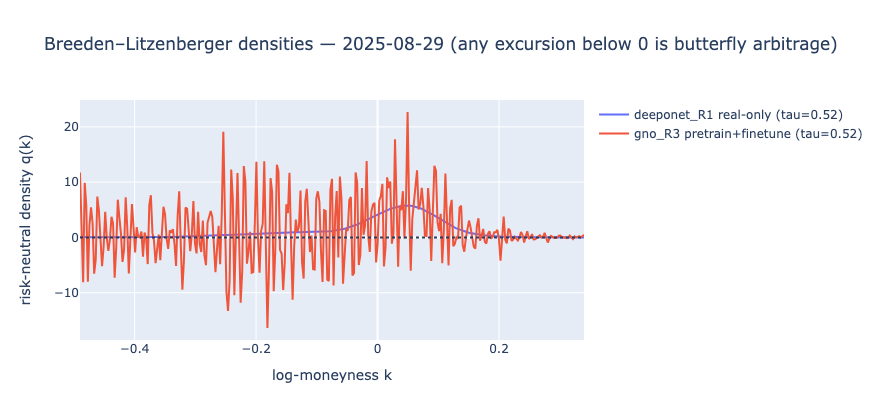
\includegraphics[width=0.95\textwidth]{figures/nb05_c08_1.png}
    \caption{Breeden--Litzenberger densities on 2025-08-29 at $\tau=0.52$. The DeepONet's
    density is smooth and nonnegative; the GNO's oscillates around it and crosses
    below zero repeatedly, giving the negative mass reported in Table~\ref{tab:density}. Any
    excursion below the dashed line is butterfly arbitrage. Source: Notebook 05, \S C.}
    \label{fig:nb05densities}
\end{figure}

% ============================================================================
\section{A static-arbitrage scanner on bid/ask quotes}\label{sec:scanner}
% ============================================================================

The audits so far interrogate fitted surfaces. This section scans the raw quotes instead,
asking per day and per (expiry, type) whether the quoted bid/ask system already contains
executable static arbitrage, that is, whether the market itself violates
Proposition~\ref{prop:shape} when priced at the touch. The same checks are run at mid prices
alongside, and the gap between the two columns is the bid-ask spread absorbing the apparent
violations. This gives us the data-level baseline against which model violation rates must be
read, since a model cannot be blamed for reproducing an arbitrage the quotes contain.

\paragraph{Tests.} Per (expiry, type) side, strikes ascending:
\begin{enumerate}[label=(S\arabic*)]
\item \emph{Vertical (monotonicity):} calls must be non-increasing in $K$, puts
non-decreasing; the executable flag is $C^{\mathrm{bid}}(K_{i+1})>C^{\mathrm{ask}}(K_i)$
(sell the spread, collect a positive premium against a nonnegative payoff;
Proposition~\ref{prop:shape}(a), monotone part), and symmetrically for puts.
\item \emph{Butterfly (convexity):} for consecutive strike triples $K_1<K_2<K_3$ with
weights $\lambda_1=(K_3-K_2)/(K_3-K_1)$, $\lambda_3=(K_2-K_1)/(K_3-K_1)$, the executable
flag is $\lambda_1C^{\mathrm{ask}}(K_1)-C^{\mathrm{bid}}(K_2)+\lambda_3C^{\mathrm{ask}}(K_3)<0$
(buy the wings at the ask, sell the body at the bid;
Proposition~\ref{prop:shape}(a), convex part).
\end{enumerate}
Counts are reported per day, in absolute terms and as a share of checks, together with the
premium locked by executable violations in index points, and stored in
\texttt{nb05\_static\_arb.parquet} alongside the per-day model audit columns so that
data-level and model-level rates can be compared directly.

\paragraph{Results.} Over $1{,}926$ trading days the scanner checks roughly $1.22\times10^7$
vertical pairs and $1.21\times10^7$ butterfly triples. At the touch it finds \textbf{62
executable violations} ($6$ vertical, $56$ butterfly) on \textbf{$43$ days} ($2.2\%$), locking
a cumulative premium of $18.3$ index points over eight years. The SPX quote system is
therefore, to first order, free of executable static arbitrage. The mid-price count is larger
by orders of magnitude ($2.5\times10^4$ vertical and $2.6\times10^6$ butterfly flags, with at
least one on every single day), and the whole difference is the bid-ask spread: the violations
a mid-quote surface would report are not transactable.

This is the baseline the model audits must be read against, and it is the counterpart of the
detection-power result in \S\ref{sec:power}. The same market whose residuals sit below the
net-profitability frontier is the market whose quotes admit essentially no executable static
arbitrage. The $43$ flagged days concentrate in the ultra-short bucket, the same bucket where
fitted-SVI violations concentrate (Table~\ref{tab:buckets}), which suggests that part of the
short-end difficulty is in the data rather than in the smoother.

% ============================================================================
\section{Residual relative value: economic significance rather than alpha}\label{sec:residual}
% ============================================================================

\paragraph{This is not an arbitrage.} The strategy studied here is relative value, in the sense
of Section~\ref{sec:twoquestions}. An arbitrage has a payoff structure guaranteeing no loss in
any state, executable at quoted prices. What follows has no such structure: it ranks options by
their residual $r_i=\sigma^{\mathrm{mkt}}_i-\sigma^{\mathrm{model}}_i$, goes long the cheap tail
and short the rich tail, and profits only if residuals mean-revert on average. It can lose in
any given period. We therefore test economic significance rather than alpha, and report the
result as a comparison between a clean and a deliberately arbitrage-dirty surface on identical
universes with identical costs. The question is whether the residuals carry economic
information, and whether arbitrage-dirtiness degrades it.

\paragraph{Protocol.} Per (day, family), residuals are computed on held-out, in-domain quotes
and matched to $t+h$ by (\texttt{exdate},\,strike). Two layers follow. The information layer
reports $$\mathrm{IC}=\mathrm{Spearman}(r_t,-\Delta\mathrm{IV}_{t\to t+1})$$ and a decile spread
net of entry half-spreads. The backtest uses a common universe per day, made of held-out quotes
inside every model's domain with finite cost capped at $5\,\vp$, so that names and costs are
identical across models and only the surface differs. Ranking is bucket-neutral
($\tau$-terciles $\times$ $|k|$-terciles), with an entry filter that trades only quotes
mispriced beyond their own half-spread. We sweep holding horizons $h\in\{1,3,5,10\}$ and an
execution ladder from touch (full spread paid) through half to mid (none), where mid bounds
what a market maker could capture and touch is what a taker pays. P\&L is first-order vega, one
round trip per holding period, non-overlapping, fit-gated at $5\,\vp$ day RMSE, with real
per-name half-spreads converted through Black vega. The counterfactual is the same day smoothed
with $\lambda=10$ and with $\lambda=0$.

\paragraph{Information layer.} On the controlled synthetic validation, where quote noise
mean-reverts by construction, the pipeline behaves as designed: IC $0.712$ for the clean
surface against $0.455$ for the dirty one, on the same day and quotes. On the real staging days
the ICs are small and unstable in sign, as they must be at this sample size (DeepONet $-0.62$
to $+0.37$; GNO $\approx0$; SSVI $-0.61$ to $+0.36$), and the single real clean-versus-dirty day
is statistically indistinguishable (IC $0.260$ against $0.277$). At $n=10$ days this layer
validates the pipeline; it is not evidence.

\begin{table}[htbp]\centering\small
\caption{Backtest, mean net P\&L per holding period (\vp), staging sample (deep rows:
one period, 2018-01-08; operator and SSVI rows: the ten 2025-08 days). Sharpe, drawdown and hit
rate are computed and stored (\texttt{nb05\_backtest\_stats.parquet}) but are meaningless at
$n_{\mathrm{periods}}\le10$; the production run populates them.
Source: Notebook 05, \S F2.}
\label{tab:f2}
\begin{tabular}{lcccc@{\qquad}cccc}
\toprule
 & \multicolumn{4}{c}{execution = touch} & \multicolumn{4}{c}{execution = mid} \\
Model & $h{=}1$ & $3$ & $5$ & $10$ & $h{=}1$ & $3$ & $5$ & $10$ \\
\midrule
Deep ($\lambda{=}10$) & $-2.06$ & $-1.36$ & $-1.29$ & $-0.58$ & $+0.08$ & $+0.45$ & $+0.61$ & $+1.12$ \\
Deep ($\lambda{=}0$, dirty) & $-2.10$ & $-1.57$ & $-1.45$ & $-1.23$ & $+0.05$ & $+0.30$ & $+0.59$ & $+0.75$ \\
DeepONet R1 & $-0.74$ & $-0.79$ & $-1.24$ & n/a & $-0.05$ & $-0.15$ & $-0.69$ & n/a \\
GNO R3 & $-0.67$ & $-0.81$ & $-1.17$ & n/a & $-0.06$ & $-0.28$ & $-0.67$ & n/a \\
SSVI & $-0.75$ & $-1.09$ & $-1.53$ & $-1.78$ & $+0.01$ & $-0.01$ & $-0.14$ & $-0.09$ \\
\bottomrule
\end{tabular}
\end{table}

Despite the small sample, two descriptive patterns are consistent across the staging results.
First, no model produces positive net P\&L under touch execution at any holding horizon. Where a
residual signal exists, it is therefore too small to compensate for the bid--ask spread.
Section~\ref{sec:power} shows that this is not simply a failure of the detection pipeline.

Second, the clean surface outperforms its arbitrage-dirty counterpart in all eight matched
horizon--execution cells. At mid execution, for example, the ten-day result is $+1.12\,\vp$ for
the clean surface against $+0.75\,\vp$ for the dirty one, with the universe and
transaction-cost assumptions held fixed.

\begin{finding}[Staging observation: arbitrage-dirtiness weakens the residual signal]
\label{find:economics}
On matched counterfactuals (same day, quotes, universe, costs), the residual signal computed
against an arbitrage-dirty surface is weaker than against its clean twin: IC $0.455$ against
$0.712$ on the synthetic validation, and lower net P\&L in $8/8$ backtest cells on the single
real staging day. Those eight cells are not independent and the synthetic IC is not market
evidence, so this is recorded as a validation of the pipeline rather than as a result: the
machinery detects the direction it was built to detect, and statistical confirmation is left to
the production run.
\end{finding}

\begin{figure}[H]
    \centering
    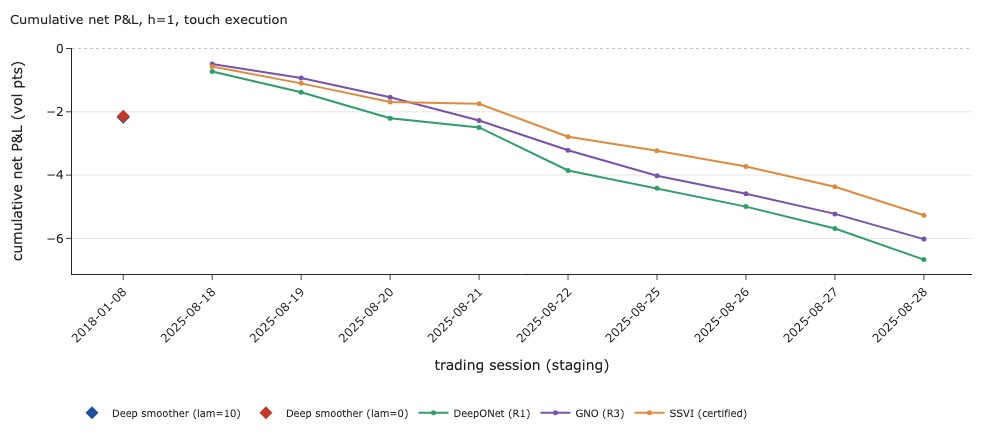
\includegraphics[width=0.95\textwidth]{figures/nb05_f2_cumulative.png}
    \caption{Cumulative net P\&L at $h=1$ with touch execution, cumulated over the nine trading
    sessions common to the three 2025 families. Every family loses steadily, the first of the two
    patterns of \S\ref{sec:residual} in visual form. The two deep-smoother entries have a single staging period (2018-01-08) and
    appear as one overlapping marker on the left, their constrained and unconstrained P\&L being
    almost identical on that day. Source: Notebook 05, \S F2.}
    \label{fig:nb05f2}
\end{figure}



% ============================================================================
\section{Detection power: the net-profitability frontier of this market}\label{sec:power}
% ============================================================================

Section~\ref{sec:residual} showed that the observed residual signal is not profitable after
paying the spread. That result alone does not tell us whether the signal is genuinely too weak
or whether the backtest simply lacks the power to detect it. The purpose of this section is
therefore to calibrate the smallest synthetic signal that the same pipeline could detect and
monetise under the observed market conditions. Comparing the empirical residuals with that
detection frontier allows us to distinguish between a limitation of the pipeline and a
limitation imposed by transaction costs.

\paragraph{Protocol.} Take a real day (2025-08-28; universe $1{,}760$ names with real
per-name half-spreads) and inject a synthetic mispricing of amplitude $a$ (vol points,
random sign) into $10\%$ of names, decaying toward the surface with half-life $h$ (trading
days). The injected residuals go through the same backtest machinery as
Section~\ref{sec:residual}, with the same entry filter, bucket-neutral deciles and real costs,
and we compute annualised net Sharpe at the touch over the best holding horizon, across $120$
replications per $(a,h)$ cell. Two calibrations keep the exercise honest. The observation noise
through which the signal must be detected is the robust dispersion of actual residuals
($\sigma_{\mathrm{obs}}=3.92\,\vp$), and the outcome noise is the robust dispersion of actual
matched day-over-day IV moves net of per-expiry common shifts
($\sigma_\varepsilon=0.09\,\vp$/day, idiosyncratic).

\paragraph{Results.} At the touch, a mispricing must have amplitude $\ge3.0\,\vp$ with a
half-life of $5$ days or less, rising to $\ge5.0\,\vp$ at half-lives of $8$--$12$ days, to be
net-profitable: longer persistence raises the amplitude required rather than lowering it. The
pipeline validation passes: an injected signal with $a=5\,\vp$ and a $12$-day half-life produces
an annualised Sharpe of $18.4$, so the machinery does detect large persistent signals and the
empty real-data result of Section~\ref{sec:residual} is a property of the market rather than of
the code. Against this frontier, the empirical residual distribution of the same day has
$98.1\%$ of quotes beyond their own half-spread, but a median exceedance of only $2.55\,\vp$ and
a day-1 residual autocorrelation of $+0.90$ (half-life $\approx6.9$ trading days). The empirical
point therefore sits below the $3$--$5\,\vp$ breakeven contour. The margin is narrow, roughly
half a volatility point at the measured persistence, so the conclusion is that this market
prices the residual signal out, not that it does so by a wide margin.

\begin{finding}[The spread prices out the residual signal]\label{find:frontier}
On real SPX spreads and measured noise, a residual mispricing must exceed $\approx3\,\vp$ with
multi-day persistence to clear touch costs, and the market's empirical residuals (median
exceedance $2.55\,\vp$, half-life $\approx7$d) sit below that frontier, though by a narrow
margin. The absence of net alpha at the touch is therefore a property of the market's spread
structure, consistent with the scanner result of Section~\ref{sec:scanner}, and not an artefact
of the pipeline, which does detect signals above the frontier.
\end{finding}

\begin{figure}[htbp]
    \centering
    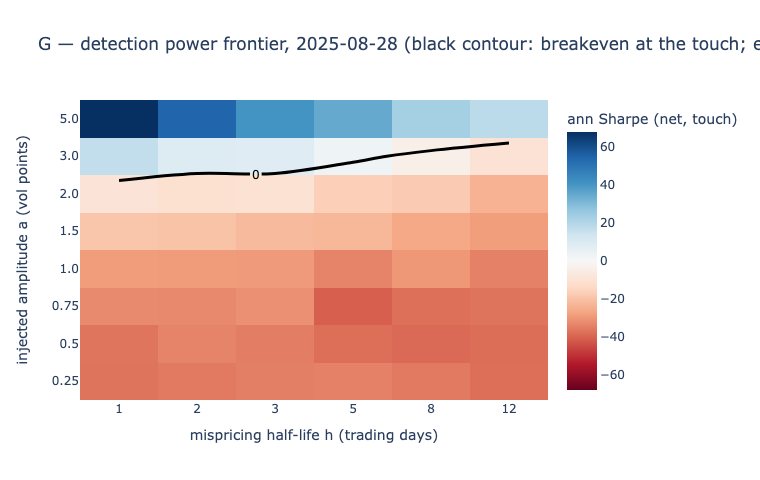
\includegraphics[
        width=0.80\textwidth,
        trim=0cm 1.3cm 0.8cm 3.5cm,
        clip
    ]{figures/nb05_g_frontier.png}
    \caption{Annualised net Sharpe at the touch as a function of the injected amplitude $a$ and
    half-life $h$. The black line is the breakeven contour, labelled with the Sharpe value it
    traces, namely zero; the region above it is net-profitable. Both axes are categorical, so
    their columns are equally spaced rather than to scale. The market's empirical residuals for
    this day, with median exceedance $2.55\,\vp$ and half-life $\approx7$ days, fall below the
    contour, as discussed in the text. Source: Notebook 05, \S G.}
    \label{fig:nb05g}
\end{figure}
% ============================================================================
\section{Unified evaluation and discussion}\label{sec:unified}
% ============================================================================

\subsection{One table, four questions}

\begin{table}[htbp]\centering
\caption{The unified view. Fit is hold-out IV RMSE under the shared $\mathrm{crc32}$
protocol (NB02: 8-day staging; NB03: staging days, endpoint-certified calibrator of
Remark~\ref{rem:cert}; NB04: 386 chronological out-of-sample days). The DeepONet row is the
real-only regime R1 in every column, so that its fit, audit and downstream entries describe the
same model. Audit columns are \emph{material} rates on grids independent of any penalty grid.
Downstream columns from this chapter (staging days). Cost is per new day on CPU.}
\label{tab:unified}
\resizebox{\textwidth}{!}{%
\begin{tabular}{lcccccc}
\toprule
 & Fit, hold-out (\vp) & Guarantee & Material viol.\ (audit) & LV repair & Density neg.\ mass & Cost / day \\
\midrule
SVI (per slice)      & $0.64$ & none (audited ex post) & 12\% of slices & n/a (no $\partial_\tau w$) & slice-level $g<0$ & $\sim$1\,s \\
SSVI (certified)     & $1.91$ & \textbf{theorem} (Thm.~\ref{lem:range}) & 0\% & 0\% & 0\% & $\sim$1\,s \\
Deep ($\lambda{=}10$)& $1.15$--$1.31$ & soft + certified prior & 0\% (staging) & 0\% & 0\% & 80--100\,s \\
DeepONet (R1)        & $2.69$ & soft, train days only & $0.056\%$ (cal) & 0.0--0.6\% & $\approx0$ & $<$1\,ms \\
DeepONet $+$ prior   & $\mathbf{1.32}$ & soft $+$ certified prior & $\mathbf{0.0\%}$ & 0\% & 0\% & $<$1\,ms$+$1\,s \\
GNO (R3, best fit)   & $1.26$ & soft, train days only & \textbf{21.8\% (bfly)} & \textbf{48--50\%} & up to \textbf{230\%} & 40--400\,ms \\
\bottomrule
\end{tabular}}
\end{table}

Table~\ref{tab:unified} answers the four questions this thesis asks of any smoother.

\paragraph{How well does it fit?} Per-slice SVI still leads on the staging sample, while the
deep smoother and GNO both lie inside the SVI--SSVI window defined in
Section~\ref{sec:parametric}. The operator does so at amortised cost, which is the point of
learning the smoothing map rather than refitting it daily.

\paragraph{What does it guarantee, and on what set?} Only SSVI, and hence the deep
smoother's prior, carries a theorem. A soft penalty guarantees nothing beyond the grid on which
it was evaluated, and for an operator nothing beyond the training days. That distinction, not
the penalty weight, separates the two halves of the table.

\paragraph{What does a failure cost?} This chapter measured that directly. The GNO buys
its fit advantage with a local-variance surface invalid on half its domain,
risk-neutral densities with up to $230\%$ negative mass, and day-to-day instability of
around $8\,\vp$. The unreported path-dependent experiment noted in the conclusion points
the same way, more sharply, but is not counted here.

\paragraph{What does it cost to run?} The operators are four orders of magnitude faster per day
than the per-day smoother, a genuine advantage. The GNO's main benefit is therefore
computational speed, but this comes with weaker no-arbitrage control on unseen days. The
prior-embedded operator avoids this trade-off here, combining fast evaluation with clean audits.

\subsection{What we would tell a desk}

\begin{enumerate}[label=(\roman*),leftmargin=*]

\item \textbf{Do not rely on a model's in-sample violation report alone.} A soft-constraint
model is naturally evaluated on the grid where its penalty was imposed, so a low violation rate
there says little about behaviour elsewhere. The relevant comparison is between training nodes
and an independent audit grid, together with the material violation rate.

\item \textbf{Use a certified prior multiplicatively when one exists.} The prior provides the
protection and the corrector adds accuracy, without trading one against the other
(Tables~\ref{tab:ablation} and~\ref{tab:prioroperator}).

\item \textbf{Project an operator's output before using it downstream.} If an unconstrained
operator is retained for speed, its output should be projected or recalibrated onto an
arbitrage-controlled family, for example using the repairs of Section~\ref{sec:parametric},
before any Greek or density is computed; a dedicated projection step is a natural extension.
Monte-Carlo repricing should not be the sole diagnostic, since pre-simulation repair can mask
violations in the original surface (\S\ref{sec:localvol}).

\item \textbf{Score smoothers on more than IV RMSE.} Repair rate, density mass and
day-over-day stability rank the families differently from the fit column, with the ranking
inverting more than once.

\item \textbf{Do not expect smoothing residuals to pay the touch on SPX.} The breakeven
frontier is $3$ to $5\,\vp$, while market residuals lie below it
(Finding~\ref{find:frontier}). Their value is in marking and market-making, where mid-execution
capture makes surface cleanliness worth about $+0.4\,\vp$ per ten-day period on the staging
counterfactual.

\item \textbf{Treat cleanliness as a requirement for path-dependent books.} A trajectory-dependent
payoff integrates the surface where quotes do not constrain it, precisely where soft penalties
are least reliable. A surface indistinguishable from a certified one on the vanilla objective
can still misprice and mis-hedge an exotic. Project it before it reaches the book, not after
P\&L exposes the problem.

\end{enumerate}